\documentclass{report}
\usepackage[utf8]{inputenc}
\usepackage[francais]{babel}
\usepackage[T1]{fontenc}
\usepackage{lmodern}
\usepackage{textcomp}
\usepackage{listings}
\usepackage{graphicx}
\usepackage{hyperref}
\usepackage{titlesec}
\usepackage{tcolorbox}
\usepackage{amsmath}
\usepackage{color}
\usepackage{multirow}
\usepackage{enumitem}
\usepackage{cite}

\setcounter{tocdepth}{5}
\setcounter{secnumdepth}{4}
\definecolor{dkgreen}{rgb}{0,0.6,0}
\definecolor{gray}{rgb}{0.5,0.5,0.5}
\definecolor{mauve}{rgb}{0.58,0,0.82}
\definecolor{gray}{rgb}{0.4,0.4,0.4}
\definecolor{darkblue}{rgb}{0.0,0.0,0.6}
\titleformat{\paragraph}
{\normalfont\normalsize\bfseries}{\theparagraph}{1em}{}
\titlespacing*{\paragraph}
{0pt}{3.25ex plus 1ex minus .2ex}{1.5ex plus .2ex}
\renewcommand{\thesection}{\Roman{section}}
\hypersetup{
    colorlinks=true,
    linkcolor=black,
    filecolor=magenta,
    urlcolor=cyan,
}
\lstnewenvironment{cc}
{
\lstset{frame=tblr,
  language=C,
  aboveskip=3mm,
  belowskip=3mm,
  showstringspaces=false,
  columns=flexible,
  basicstyle={\small\ttfamily},
  numbers=none,
  numberstyle=\tiny\color{gray},
  keywordstyle=\color{blue},
  commentstyle=\color{dkgreen},
  stringstyle=\color{mauve},
  breaklines=true,
  breakatwhitespace=true,
  tabsize=3
}}
{}

\begin{document}
\title{
  \begin{minipage}\linewidth
      \centering
      
\includegraphics[width=40mm]{resources/01.png}\vskip 20pt
      Modèle d’une propagation d’une épidémie
      \vskip 5pt
      \author{
        DRISSI Mohamed Reda \\
        \texttt{reda-mohamed@isty.uvsq.fr}
      }
    \end{minipage}
}
\maketitle
\newpage
\tableofcontents
\newpage
\section{Introduction}
Dans le cadre du module "Calcul Haute Performance et Simulation", il nous a été demandé de modéliser
le problème de la propagation d’une maladie dans une population. Le but de ce projet est de faire
différentes simulation afin de vérifier l'avantage d'une optimisation pageRank appliquée sur un
tel problème.\\

Nous avons choisi de développer notre projet en python 3.7 pour son abandance de librairies en calcul
matriciel et parce que nous le maitrisons bien. Nous utilisons la librairie networkx pour nos graphes.
Nous utilisons ensuite des matrices numpy pour représenter nos matrices de transitions.
Pour avoir les représentation graphique de nos simulation, nous utilisons la bibliothèque matplot.\\

Ce rapport est découpé en deux parties. Dans un premier temps nous aborderons la modélisation du problème.
Puis nous développerons les résultats que nous avons obtenus après simulation.
\section{Modélisation}
Le problème de la propagation d’un virus dans une population peut être assimilé au problème
de la promenade aléatoire d’un individus sur internet (d'où le choix de l'optimisation pageRank).
\vspace{3mm}
\begin{itemize}[label=$\bullet$]
  \item Internet $\rightarrow$ Une population
  \item Une page sur internet $\rightarrow$ Un individu dans la population
  \item Un promeneur $\rightarrow$ Un virus
  \item La promenade du marcheur $\rightarrow$ La propagation du virus
  \item Le rang d’une page est la probabilité de la présence du promeneur sur cette page $\rightarrow$
    Le rand est la probabilité d’être infecté par le virus durant une épidémie
\end{itemize}
\newpage
\subsection{Graphes}
Nous avons receuilli plusieurs graphes de ce \label{site}{lien}, les fichiers contiennent des listes
d'arrêtes, chaque ligne est sous la forme "a b" ou "a\hspace{1em}b" ou "a,b". Notre script peut
détecter soit un espace, ou une virgule ou une tabulation comme délimiteur.\\
Les sommets sont représentés comme des entiers, nos graphes sont dirigés, comme ça nous avons un
meilleur résultat avec l'algorithme pageRank.\\
La matrice de transition est créée depuis la matrice d'adjacence comme fait dans le cours.\\
Le calcul de l'état stationnaire se fait par une méthode itérative, nous comparons le résultat
de l'étape actuelle avec celui de l'étape précédente puis nous nous arrêtons si la différence est
faible (le seuil d'erreur est $10^{-4}$ par défaut).\\
Le test par défaut exécutera ces graphes:
\begin{table}[ht!]
\begin{tabular}{|c|c|c|c|}
  \hline
  Nom & Nb de sommets & Nb d'arrêtes & densité \\
  \hline
  email-Eu-core & 1005 & 25571 & 0.0506848\\
  \hline
  p2p-Gnutella08 & 6301 & 20777 & 0.0010467 \\
  \hline
  p2p-Gnutella09 & 8114 & 26013 & 0.0007903 \\
  \hline
  soc-sign-bitcoinalpha & 3783 & 24186 & 0.0030033 \\
  \hline
  wiki-Vote & 7115 & 103689 & 0.0040970 \\
  \hline
\end{tabular}
\end{table}
\newpage
\subsection{Spécifications de la machine utilisée}
    \begin{itemize}[label=$\bullet$]
      \item CPU :
      \href{https://ark.intel.com/products/88195/Intel-Core-i7-6700K-Processor-8M-Cache-up-to-4_20-GHz}
        {Intel Core i7}
        \begin{itemize}[label=$\ast$]
          \item Modèle: 6700K
          \item Fréquence: 4.0GHZ
          \item nombre de coeurs/nombre de threads: 4 cores/8 logical threads(HyperThreading©)
          \item Turbo boost : off
        \end{itemize}
      \item RAM : Corsair CMK16GX4M2B3000C15 Vengeance LPX 16GB DDR4 3000MHz C15 XMP 2.0
      \item Stockage : \href{http://downloadcenter.samsung.com/content/UM/201711/20171115103115156/Samsung_SSD_850_PRO_Data_Sheet_Rev_3.pdf}
          {Samsung 850 PRO SSD 512GB}
    \end{itemize}
    \subsection{Système}
      \begin{itemize}[label=$\bullet$]
      \item OS : Debian 9.8 Stretch (stable) x86\_64
      \item Kernel :  4.9.0-8-amd64
      \item Python 3.7.0
    \end{itemize}
  \subsection{Topologie du système}
    \begin{figure}[ht!]
      \centering
      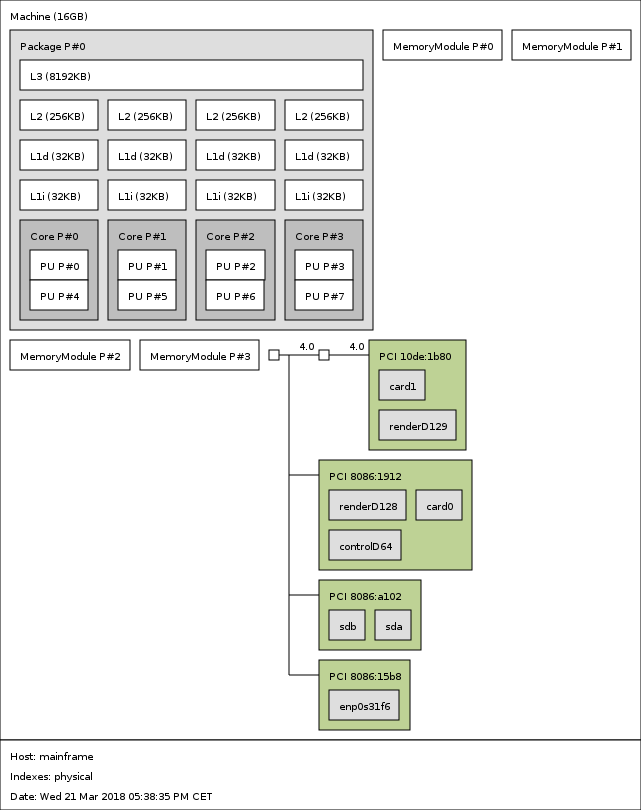
\includegraphics[scale=0.35]{resources/lstopo.png}
      \caption{Topologie générée par \href{https://manpages.debian.org/jessie/hwloc/lstopo.1.en.html}{lstopo}}
    \end{figure}
\newpage
\subsection{Paramètres de simulation}
Voici quelques paramètres que nous avons utilisé pour les différentes simulations.
\begin{itemize}[label=$\bullet$]
  \item Nombre d’itérations  = $150$
  \item Facteur de damping $\alpha = 0.8$
  \item Pourcentage de personnes infecté initialement : $x=5\%$
  \item Probabilité d’infecter un voisin : $\nu = 1 - \alpha = 0.2$
  \item Probabilité de guérir par hasard:$\gamma = 0.02$
\end{itemize}
\newpage
\section{Simulations}
\subsection{Résultats}
Nous allons utiliser le script \texttt{full.sh} qui nous calculera tous les graphes fournis,
nous avons trouvé ces graphes sur le site de snaps de Stanford~\cite{snapnets}.\\
Pour un usage granulaire, une aide est fournie (seul le nom de fichier est obligatoire):
\begin{tcolorbox}
  \begin{verbatim}
bash~$  cd src
bash~$  python -m app.main -h
usage: main.py [-h] [-g FILENAME] [-i INFECTED] [-v RANDOM_VACCINATION]
               [-H HEAL] [-c CONTAMINATION] [-t ITER]

Simple epidemic modeling example using PageRank

optional arguments:
  -h, --help            show this help message and exit
  -g FILENAME, --input-graph FILENAME
                        File containing the edge list of the matrix
                        to process
  -i INFECTED, --infected INFECTED
                        Ratio of initially randomly individuals
  -v RANDOM_VACCINATION, --vaccinate RANDOM_VACCINATION
                        Ratio of initially randomly vaccinated individuals
  -H HEAL, --heal HEAL  Probability of randomly healing when infected
  -c CONTAMINATION, --contamination CONTAMINATION
                        Probability of contaminating each neighbor when
                        infected
  -t ITER, --iteration ITER
                        Number of iterations of the simulation
  \end{verbatim}
\end{tcolorbox}
\subsubsection{email-Eu-core.txt}
The network was generated using email data from a large European research institution
Réseau généré avec les données mail d'une institution de recherche européenne.
\begin{tcolorbox}
  \begin{verbatim}
    Name:
    Type: DiGraph
    Number of nodes: 1005
    Number of edges: 25571
    Average in degree:  25.4438
    Average out degree:  25.4438
    Density:0.050684822897464864
    Ratio of initially infected individuals:0.05
    Ratio of initially randomly vaccinated individuals:0.22
    Probability of contaminating each neighbor when infected:0.2
    Probability of randomly healing when infected:0.26
    Number of iterations:150
    Time spent to run each simulation:
      No Vaccination: 641 ms
      Random Vaccination: 374 ms
      PageRank Vaccination: 391 ms
  \end{verbatim}
\end{tcolorbox}
\begin{figure}[ht!]
  \centering
  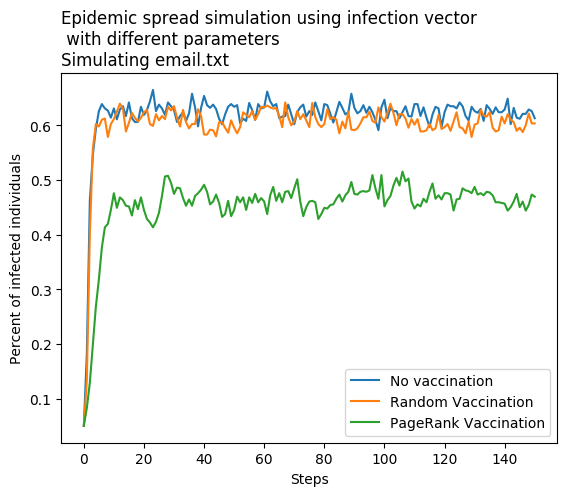
\includegraphics[scale=0.7]{../plots/email.png}
  \caption{Graphe de simulation email-Eu-core}
\end{figure}
\newpage
\subsubsection{p2p-Gnutella08.txt}
Réseau de partage de fichiers Gnutella en P2P d'août 2002
\begin{tcolorbox}
  \begin{verbatim}
    Name:
    Type: DiGraph
    Number of nodes: 6301
    Number of edges: 20777
    Average in degree:   3.2974
    Average out degree:   3.2974
    Density:0.0010467978123905755
    Ratio of initially infected individuals:0.05
    Ratio of initially randomly vaccinated individuals:0.22
    Probability of contaminating each neighbor when infected:0.2
    Probability of randomly healing when infected:0.26
    Number of iterations:150
    Time spent to run each simulation:
    No Vaccination: 14 seconds 744 miliseconds
    Random Vaccination: 3 seconds 276 miliseconds
    PageRank Vaccination: 974 miliseconds
  \end{verbatim}
\end{tcolorbox}
\begin{figure}[ht!]
  \centering
  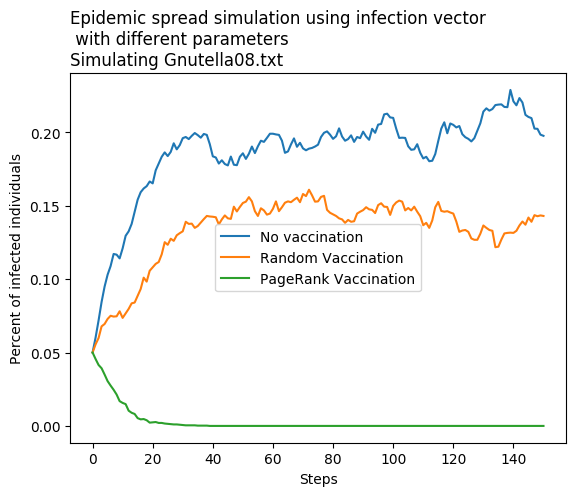
\includegraphics[scale=0.7]{../plots/Gnutella08.png}
  \caption{Graphe de simulation p2p-Gnutella08}
\end{figure}
\newpage
\subsubsection{p2p-Gnutella09.txt}
Réseau de partage de fichiers Gnutella en P2P d'août 2002
\begin{tcolorbox}
  \begin{verbatim}
    Name:
    Type: DiGraph
    Number of nodes: 8114
    Number of edges: 26013
    Average in degree:   3.2059
    Average out degree:   3.2059
    Density:0.0007903217921884197
    Ratio of initially infected individuals:0.05
    Ratio of initially randomly vaccinated individuals:0.22
    Probability of contaminating each neighbor when infected:0.2
    Probability of randomly healing when infected:0.26
    Number of iterations:150
    Time spent to run each simulation:
    No Vaccination: 25 seconds 538 miliseconds
    Random Vaccination: 7 seconds 89 miliseconds
    PageRank Vaccination: 1 seconds 549 miliseconds
  \end{verbatim}
\end{tcolorbox}
\begin{figure}[ht!]
  \centering
  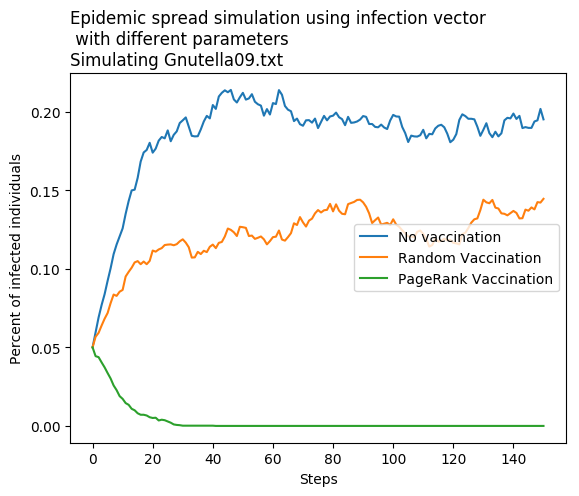
\includegraphics[scale=0.7]{../plots/Gnutella09.png}
  \caption{Graphe de simulation p2p-Gnutella09}
\end{figure}
\newpage
\subsubsection{soc-sign-bitcoinalpha.csv}
Réseau représentant les personnes se faisant confiance dans un échange de bitcoins sur la plateforme
bitcoin-alpha.
\begin{tcolorbox}
  \begin{verbatim}
    Name:
    Type: DiGraph
    Number of nodes: 3783
    Number of edges: 24186
    Average in degree:   6.3933
    Average out degree:   6.3933
    Density:0.0033809299947872786
    Ratio of initially infected individuals:0.05
    Ratio of initially randomly vaccinated individuals:0.22
    Probability of contaminating each neighbor when infected:0.2
    Probability of randomly healing when infected:0.26
    Number of iterations:150
    Time spent to run each simulation:
    No Vaccination: 11 seconds 582 miliseconds
    Random Vaccination: 4 seconds 650 miliseconds
    PageRank Vaccination: 1 seconds 354 miliseconds
  \end{verbatim}
\end{tcolorbox}
\begin{figure}[ht!]
  \centering
  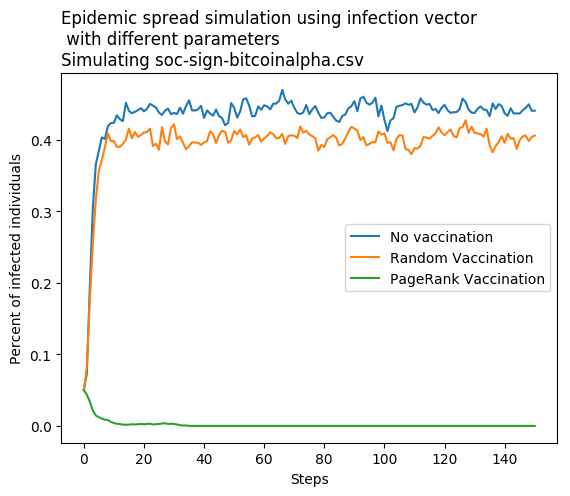
\includegraphics[scale=0.7]{../plots/soc-sign-bitcoinalpha.png}
  \caption{Graphe de simulation soc-sign-bitcoinalpha}
\end{figure}
\newpage
\subsubsection{wiki-Vote.txt}
Réseau représentant les votes entre les différents utilisateurs de wikipedia.
\begin{tcolorbox}
  \begin{verbatim}
    Name:
    Type: DiGraph
    Number of nodes: 7115
    Number of edges: 103689
    Average in degree:  14.5733
    Average out degree:  14.5733
    Density:0.004097075022161917
    Ratio of initially infected individuals:0.05
    Ratio of initially randomly vaccinated individuals:0.22
    Probability of contaminating each neighbor when infected:0.2
    Probability of randomly healing when infected:0.26
    Number of iterations:150
    Time spent to run each simulation:
    No Vaccination: 22 seconds 609 miliseconds
    Random Vaccination: 12 seconds 966 miliseconds
    PageRank Vaccination: 1 seconds 993 miliseconds
  \end{verbatim}
\end{tcolorbox}
\begin{figure}[ht!]
  \centering
  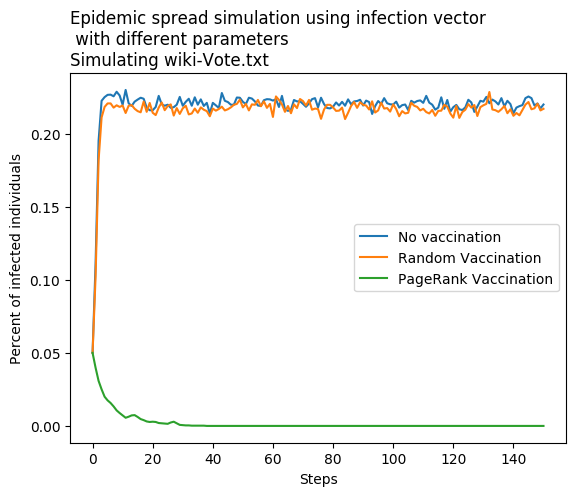
\includegraphics[scale=0.7]{../plots/wiki-Vote.png}
  \caption{Graphe de simulation wiki-Vote}
\end{figure}
\section{Analyses}
Nous remarquons l'importance de l'optimisation pageRank dans presque tous les exemples, les graphes
ont la même allure, et change drastiquement le résultat, nous remarquons aussi que les vaccinations
aléatoires génère un graphe à allure similaire à celui de la non vaccination. Donc sur un échantillon
assez important nous ne remarquerons donc pas de différence.\\
Le changement du pourcentage de vaccination vers $0.12$ et $0.32$ ne change pas l'allure du résultat.\\
À chaque fois, l'algorithme pageRank commence à se stabiliser entre les itérations 20 et 40, si
le pourcentage de vaccination est de $22\%$. Quand nous augmentons ce pourcentage, cette stabilisation
peut changer mais que légèrement.
\section{Conclusion}
Pour conclure, les simulations faites durant ce projet ne permettent pas de représenter la réalité.
Les paramètres que nous avons choisi de fixer ne sont pas suffisants, il faut prendre en compte
plusieurs autres variables(la probabilité de tomber malade en ayant quand même le vaccin,
la probabilité d’être contaminé n'est pas la même pour tous les individus, les pénuries, le coût du
vaccin, l'habilité à vacciner des individus, etc).
\bibliography{bib}{}
\bibliographystyle{plain}

\end{document}
